\section{Two-DOF Quarter Car Model}
To analyze the parameters related to the suspension system, a simplified quarter-car model, as shown in \ref{fig:m1}(a), was utilized. The quarter-car model was chosen due to its simplicity and common use in analyzing the vertical vibrations caused by railway disturbances in vehicle dynamic models.

The vehicle's mass is divided into two: the sprung mass (representing the vehicle body) and the unsprung mass (tire). Suspension springs and dampers connect the sprung and unsprung masses and the road.

Both the transverse and longitudinal deflections are considered insignificant compared to the vertical deflections of the suspension system. For the passive suspension system, the actuator force is not considered as there is no control element, as shown in \ref{fig:m1}(b).

\begin{figure}[H]
	\centering
	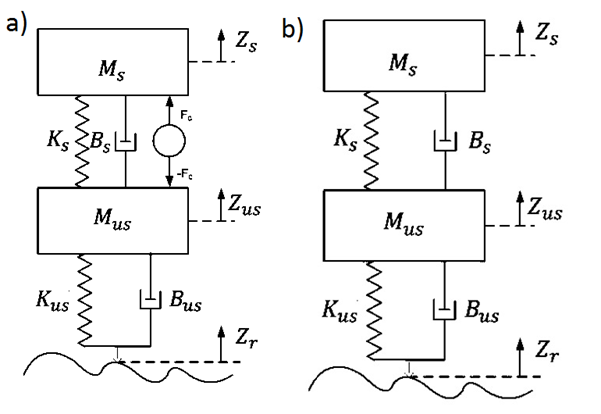
\includegraphics[width=0.4\linewidth]{model1.png}
	\caption{Active suspension system (a) and Passive suspension (b).}
	\label{fig:m1}\cite{lqr_acti}
\end{figure}

\begin{table}[H]
	\centering
	\caption{Parameters of Quarter Car Model.}
	\begin{tabular}{l|l}
		\hline
		$M_s$ & Vehicle body mass or sprung mass. \\
		$M_{us}$ & Unsprung mass (Tire, wheel, brake caliper, suspension links, etc.) \\
		$K_s$ & Spring constant for the sprung mass. \\
		$K_{us}$ & Spring constant for the unsprung mass. \\
		$B_s$ & Inherent damping coefficient for the suspension system. \\
		$B_{us}$ & Inherent damping coefficient for vehicle wheel assembly. \\
		$F_c$ & The active suspensions actuator control force. \\
		$Z_s$ & Vehicle (sprung mass) body displacement. \\
		$Z_{us}$ & Vehicles wheel displacement and the unsprung masses displacement \\
		$Z_r$ & Excitation due to the railway disturbance. \\
		\hline
	\end{tabular}
	\label{table:qcm_image}
\end{table}

\newpage
\subsection{Passive Suspension Model}
The parameters for the PSS are given in the following table:

\begin{table}[h]
	\centering
	\caption{Passive Model Parameters}
	\begin{tabular}{lccc}
		
		\hline
		\textbf{Parameter} & \textbf{Symbol} & \textbf{Value}  & \textbf{Unit}  \\
		\hline
		
		Sprung mass & \( M\)& 30 & kg\\
		Unsprung mass & \( m \)& 13 & kg\\
		Spring stiffness & \( k \)& 6921 & N/m\\ 
		Tire stiffness & \( k_{t} \)& 81000 & N/m\\
		Damper average damping coefficient & \( b_{s} \)& 900 & N s/m\\
		Tire damping coefficient & \( b_{tr} \)& 0 & N s/m\\
		
		\hline
		\label{table:Parameter}
	\end{tabular}
\end{table}
\begin{figure}[H]
	\centering
	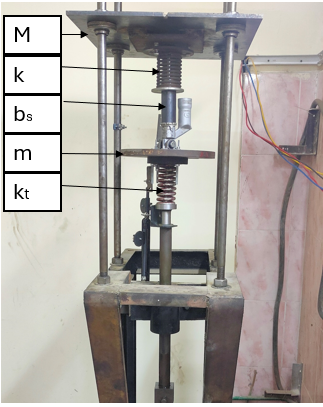
\includegraphics[width=0.45\textwidth]{layout labeled.png}
	\caption{PSS Physical Model, by Ain Shams Univresity Students as Graduation Project, Fall 2024, Automotive Department.}
	\label{fig:Passive layout}
\end{figure}

\newpage
\subsection{Active Suspension Model}
The parameters of the modified system is listed in the table below.

\begin{table}[h]
	\centering
	\caption{Active Model Parameters}
	\begin{tabular}{lccc}
		
		\hline
		\textbf{Parameter} & \textbf{Symbol} & \textbf{Value}  & \textbf{Unit}  \\
		\hline
		
		Sprung mass & \( M \)& 34 & kg\\
		Unsprung mass & \( m \)& 11 & kg\\
		Spring stiffness & \( k \)& 6921 & N/m\\ 
		Tire stiffness & \( k_{t} \)& 81000 & N/m\\
		\hline
		\label{table:Parameter}
	\end{tabular}
\end{table}

The setup of the modified Active suspension System is shown in the following figure:

\begin{figure}[H]
	\centering
	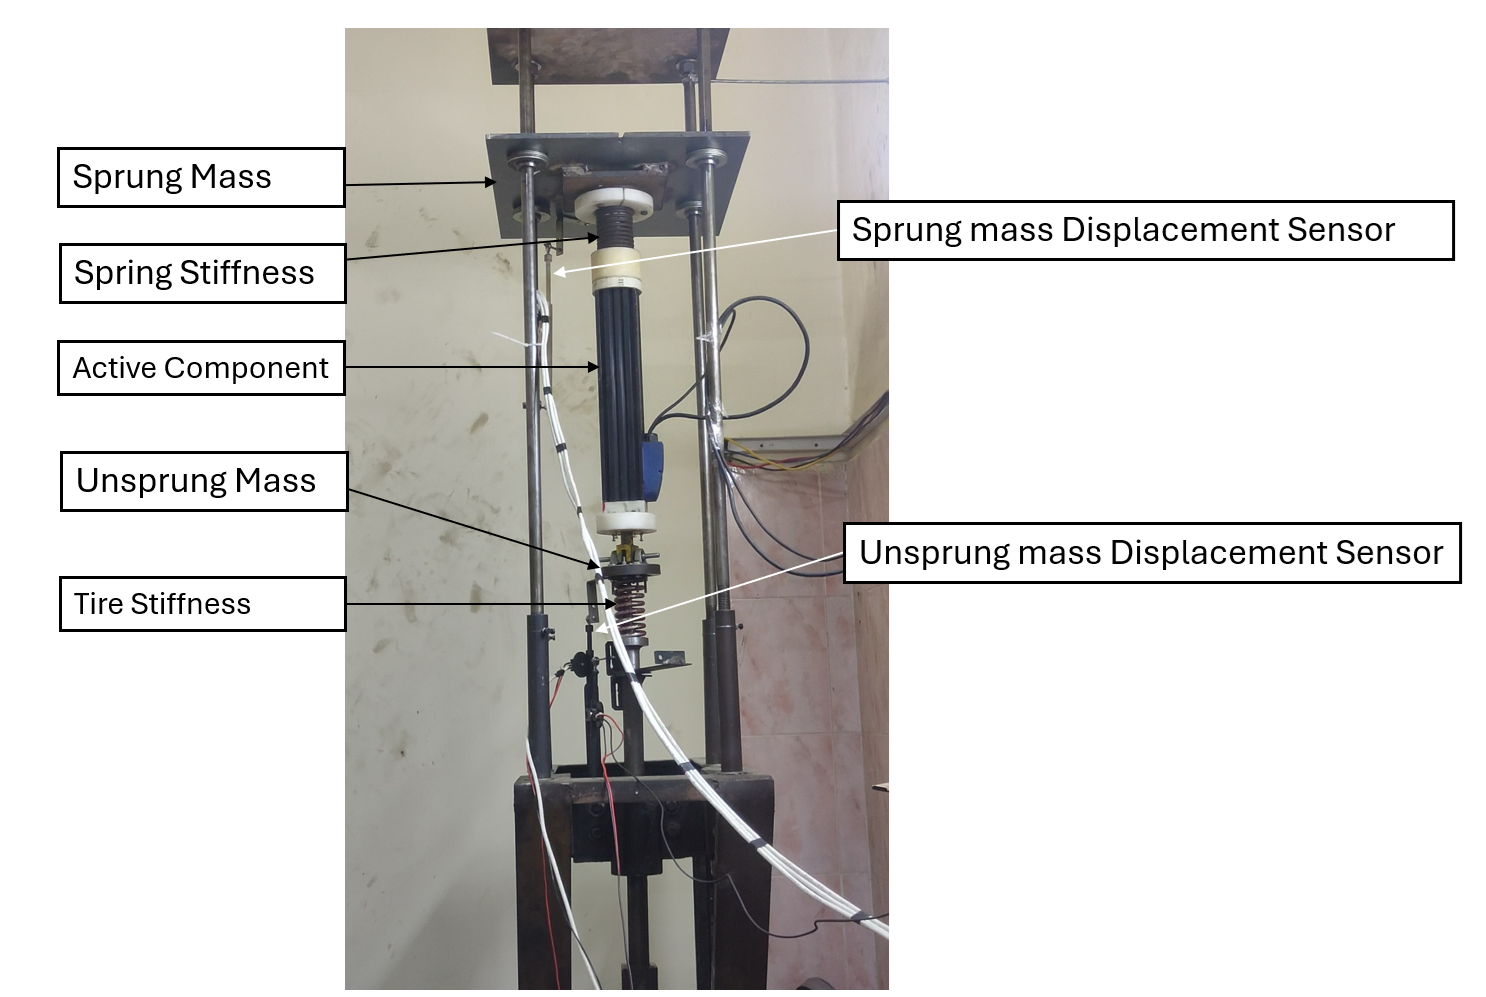
\includegraphics[width=0.9\textwidth]{Active Setup.png}
	\caption{ASS Physical Model, by Ain Shams Univresity Students as Graduation Project, Spring 2024, Automotive Department.}
	\label{fig:Active schematic diagram}	
\end{figure}


\newpage
\subsection{Equation Of Motion}

\textbf{Sprung Mass}
\begin{equation}
M_s\ddot{Z}_s = B_s\dot{Z}_{us} - B_s\dot{Z}_s - K_s(Z_s - Z_{us}) + F_c
\end{equation}

\begin{equation}
\ddot{Z}_s = \frac{B_s\dot{Z}_{us}}{M_s} - \frac{B_s\dot{Z}_s}{M_s} - \frac{K_s(Z_s - Z_{us})}{M_s} + \frac{1}{M_s}F_c
\end{equation}

\textbf{Unsprung Mass}
\begin{equation}
M_{us}\ddot{Z}_{us} = -B_s\dot{Z}_{us} - B_{us}\dot{Z}_{us} + B_s\dot{Z}_s + B_{us}\dot{Z}_r - K_s(Z_{us} - Z_s) - K_{us}(Z_{us} - Z_r) - F_c
\end{equation}\\


\begin{equation}
\ddot{Z}_{us} = -\frac{B_s\dot{Z}_{us}}{M_{us}} - \frac{B_{us}\dot{Z}_{us}}{M_{us}} + \frac{B_s\dot{Z}_s}{M_{us}} + \frac{B_{us}\dot{Z}_r}{M_{us}} - \frac{K_s(Z_{us} - Z_s)}{M_{us}} - \frac{K_{us}(Z_{us} - Z_r)}{M_{us}} - \frac{1}{M_{us}}F_c
\end{equation}\\

\subsection{State Space Model}
A state-space representation is a mathematical model used in modern control theory and system analysis to describe the behavior of a dynamic system. It offers a concise and systematic approach to representing the evolution of a system over time. In contrast to the frequency-domain representation (e.g., transfer functions), which characterizes a system's input-output relationship in terms of frequencies, the state-space representation provides a time-domain description.\\

\textbf{The general state-space representation is given by the following:}
$$\dot{x}_{(t)}=Ax_{(t)}+Bu_{(t)}$$
$$y_{(t)}=Cx_{(t)}+Du_{(t)}$$

\begin{itemize}
	\item $x$: State variables vector.
	\item $\dot{x}$: Represents the time derivative of the state variables vector.
	\item $y$: Output vector.
	\item $u$: Input vector.
	\item $A$: System matrix.
	\item $B$: Input matrix.
	\item $C$: Output matrix.
	\item $D$: Feedforward matrix.\\
\end{itemize}

\textbf{State variables:}
\begin{center}
	\begin{tabular}{|c|c|}
		\hline
		\textbf{Variable} & \textbf{Description} \\ \hline
		$X_1 = Z_s - Z_{us}$ & suspension travel \\ \hline
		$X_2 = \dot{Z}_s$ & sprung mass velocity \\ \hline
		$X_3 = Z_{us} - Z_r$ & wheel deflection \\ \hline
		$X_4 = \dot{Z}_{us}$ & wheel vertical velocity \\ \hline
	\end{tabular}
\end{center}

\newpage
\textbf{Inputs:} We will consider the input $\boldsymbol{u}$ into the system as the road disturbance velocity $\dot{Z}_r$ and the actuator input $F_c$.\\

\textbf{Outputs:} We will consider outputs $\boldsymbol{y}$ from the system as the suspension travel $Z_s-Z_{us}$ and the vehicle body (sprung mass) acceleration $\ddot{Z}_s$.\\

Using the above equations of motion, the state-space model of the active suspension system can easily be obtained and be written in the matrix form shown below:

\begin{equation}
\begin{bmatrix}
	\dot{x}_1 \\
	\dot{x}_2 \\
	\dot{x}_3 \\
	\dot{x}_4
\end{bmatrix} = 
\begin{bmatrix}
	0 & 1 & 0 & -1 \\
	-\frac{K_s}{M_s} & -\frac{B_s}{M_s} & 0 & \frac{B_s}{M_s} \\
	0 & 0 & 0 & 1 \\
	\frac{K_s}{M_{us}} & \frac{B_s}{M_{us}} & -\frac{K_{us}}{M_{us}} & -\frac{B_s + B_{us}}{M_{us}} 
\end{bmatrix}
\begin{bmatrix}
	x_1 \\
	x_2 \\
	x_3 \\
	x_4
\end{bmatrix} + 
\begin{bmatrix}
	0 & 0 \\
	0 & \frac{1}{M_{s}} \\
	-1 & 0 \\
	\frac{B_{us}}{M_{us}} & -\frac{1}{M_{us}} \\
\end{bmatrix}
\begin{bmatrix}
	\dot{Z}_r \\
	F_c
\end{bmatrix}
\end{equation}


\begin{equation}
\begin{bmatrix}
	Y_1 \\
	Y_2
\end{bmatrix} = 
\begin{bmatrix}
	1 & 0 & 0 & 0 \\
	-\frac{K_s}{M_s} & -\frac{B_s}{M_s} & 0 & \frac{B_s}{M_s} 
\end{bmatrix}
\begin{bmatrix}
	X_1 \\
	X_2 \\
	X_3 \\
	X_4
\end{bmatrix} + 
\begin{bmatrix}
	0 & 0 \\
	0 & \frac{1}{M_s}
\end{bmatrix}
\begin{bmatrix}
	\dot{Z}_r \\
	F_c
\end{bmatrix}
\end{equation}







\section{State Space Controllability}
State-space controllability refers to the ability to drive a system from any initial state to any desired state within a finite time using an appropriate control input. A linear time-invariant (LTI) system represented in state-space form, is controllable if the controllability matrix has full rank. When this condition is met, it ensures that the system's states can be influenced by the control input, enabling effective feedback control design.\newline

$\mathcal{C} = \left[ \begin{matrix}
	B & AB & A^2B & \cdots & A^{n-1}B
\end{matrix} \right]$\newline

$rank(\mathcal{C}) = n$


\begin{verbatim}
	% MATLAB script
	ms  = 34;           % Sprung Mass (kg)
	mus = 11;           % Unsprung Mass (kg)
	ks  = 6921;         % Suspension Stiffness (N/m)
	kus = 81000;        % Wheel stiffness (N/m)
	bs  = 0;            % Suspension Inherent Damping coefficient (sec/m)
	bus = 0;            % Wheel Inhenrent Damping coefficient (sec/m)
	
	%% System Dynamics for the Active Suspension system.
	A = [ 0 1 0 -1 ;
	-ks/ms -bs/ms 0 bs/ms;
	0 0 0 1; 
	ks/mus bs/mus -kus/mus -(bs+bus)/mus];
	
	B = [0  0 ; 
	0 1/ms ; 
	-1  0 ;
	bus/mus -1/mus ];
	
	C = [ 1 0 0 0 ; 
	-ks/ms -bs/ms 0 bs/ms ];
	
	D = [0 0;
	0 0;
	0 0;
	0 0;
	0 0;
	0 1/ms];
	
	%% Controllability
	rank(ctrb(A,B))
\end{verbatim}

The following figure shows that the system is controllable, because its controllability matrix is full rank which is equal to the number of states.\newline

\begin{figure}[H]
	\centering
	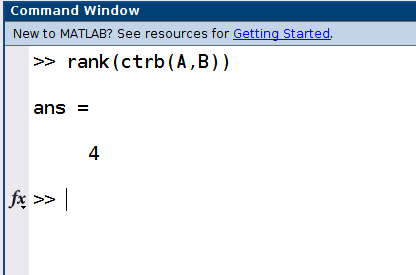
\includegraphics[width=0.4\textwidth]{ctrb.png}
	\caption{Conrollability matrix is full rank}
	\label{fig:ctrb}	
\end{figure}


\section{Road Disturbance Profile}
The slider-crank mechanism as shown in\ref{fig:sliderr} is used to simulate road. This mechanism converts the rotational motion of a crank into the linear motion of a slider, effectively replicating the vertical displacement experienced by a vehicle's suspension system when driving over uneven road surfaces which can change road amplitude by changing eccentricity from crank disk.
\begin{figure}[H]
	\centering
	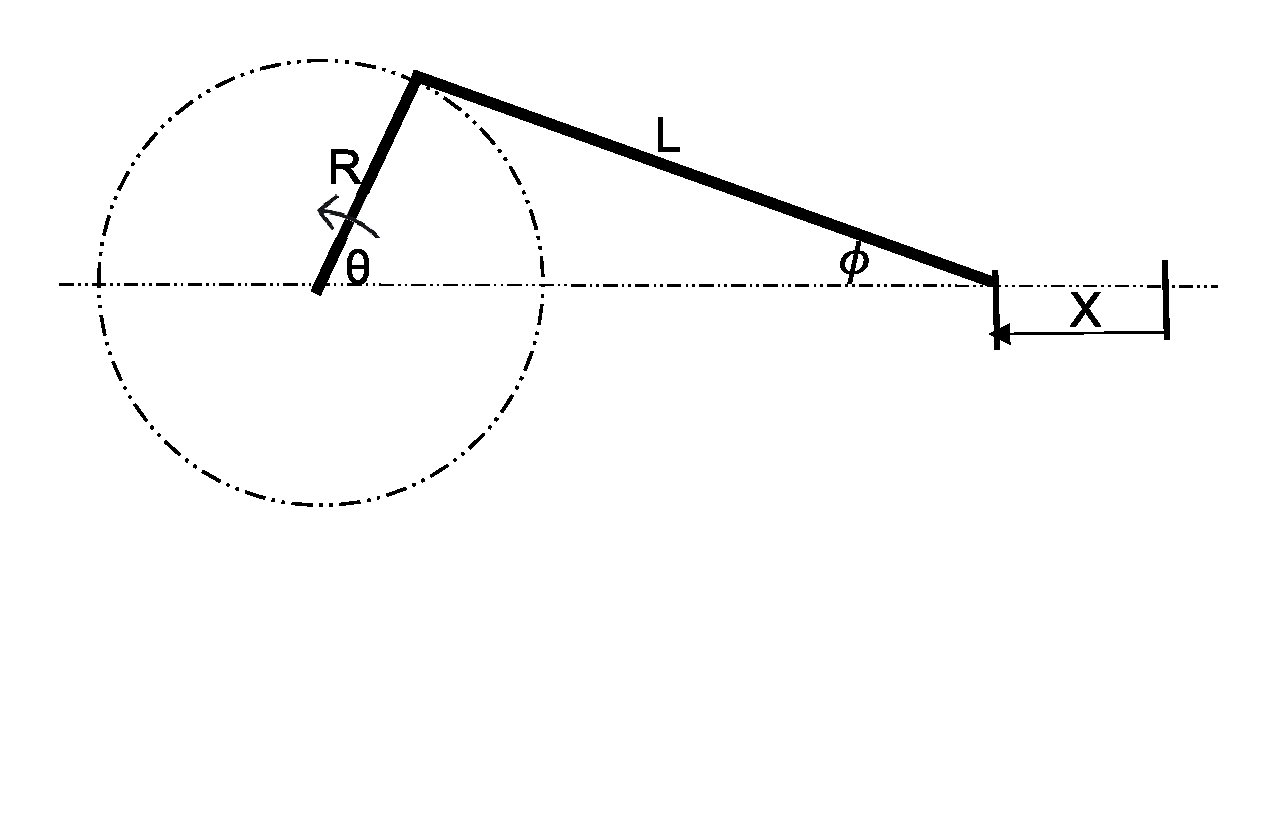
\includegraphics[trim=0cm 4cm 0cm 0cm, clip, width=1\linewidth]{sliderr.pdf}
	\caption{the slider crank mechanism}
	\label{fig:sliderr}
\end{figure}

\begin{itemize}
	\item $R$: Length of the crank
	\item $L$: Length of the connecting rod
	\item $\theta $: Angle of the crank 
	\item $x$: Position of the slider
\end{itemize}
\newpage
\subsection*{Kinematic Equations}

The position \( x \) of the slider can be determined using the crank angle \( \theta \) and \( \phi \) be the angle of the connecting rod with the horizontal. The position \( x \) of the slider can be expressed as:

\[
x = R \left[ 1 - \cos \theta + n - \sqrt{n^2 - \sin^2 \theta} \right]
\]

since \( n = \frac{L}{R} \).






%%%%%%%%%%%%%%%%%%%%%%%%%%%%%%%%%%%%%%%%%%%%%%%%%%%%%%%%%%%%%%%%%%%%%%%%%%%%

\iffalse
\section{Quarter Car Passive Suspension Model}

The vertical dynamics of the tire can be simply equated to a spring and a damping mechanism, and then the 2-DOF dynamic model as shown in figure \ref{fig:qcm} can be established.
This model is one of the most widely used suspension models, which is very important when studying vehicle dynamics, especially ride comfort and road handling characteristics. It represents the vibration behavior of the car body and the wheel. \cite{sun2020advanced}

\begin{figure}[H]
	\centering
	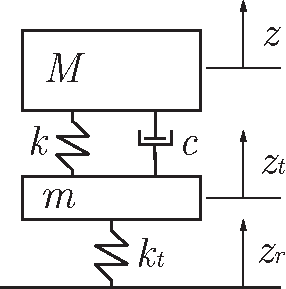
\includegraphics[width=0.4\linewidth]{qcm.pdf}
	
	\caption{Quarter Car Model\cite{researchgate_hybrid_control}.}
	\label{fig:qcm}
\end{figure}

Based on the free body diagram of the quarter car model shown in figure \ref{fig:qcm} and Newton's second law:
\begin{equation}
	m\ddot{z_t}=-k(z_t-z)-c(\dot{z_t}_-\dot{z})-k_t(z_t-z_r)
	\label{eqn:4.1}
\end{equation}
\begin{equation}
	M\ddot{z}=-k(z-z_t)-c(\dot{z}-\dot{z}_t)
	\label{eqn:4.2}
\end{equation}


\begin{table}[H]
	\centering
	\caption{Parameters of Quarter Car Model.}
	\begin{tabular}{ l|l }
		\hline
		$m$   & Unsprung mass (Tire, wheel, brake caliper, suspension links, etc.) \\
		$M$   & Quarter-car body mass                                              \\
		$k$   & Stiffness of the suspension                                        \\
		$k_t$ & Stiffness of the tire                                              \\
		$c$   & Damping coefficient of the sprung shock-absorber                   \\
		$z$   & Vertical position of the car body                                  \\
		$z_t$ & Vertical position of the unsprung mass                             \\
		$z_r$ & Vertical position of road profile                                  \\
		\hline
	\end{tabular}
	\label{table:qcm}
\end{table}


\section{Quarter Car Active Suspension Model}
With proper controlling methods, an active suspension can result in compromise
between vehicle ride comforts to road handling stableness be more improved, thus making
it an overall enhanced suspension design\cite{riduan2018review}.
Figure \ref{fig:Active schematic diagram} shows the two-degrees-of
freedom system that represents the quarter-vehicle active 
suspension model. It consists of an upper mass ($M$), 
representing the body mass (sprung mass), as well as a 
lower mass ($m$), representing the wheel mass (un-sprung 
mass), and its associated parts. The vertical motion of the 
system is described by the displacements ($z$), and($z_t$) , 
while the excitation due to road disturbance is ($z_r$). The 
suspension spring constant is ($k$), damping coefficient is 
($c$), and the tyre spring constant is ($k_t$) (the tyre damping is 
neglected). The data employed here for the quarter
vehicle system are listed in Table \ref{table:qcm}. 

Based on the free body diagram of the quarter car model shown in figure 
By applying Newton’s second law the equations of 
motion for the sprung and unsprung masses of the quarter
car suspension model are given by \cite{chiou2009using}:
\begin{figure}[H]
	\centering
	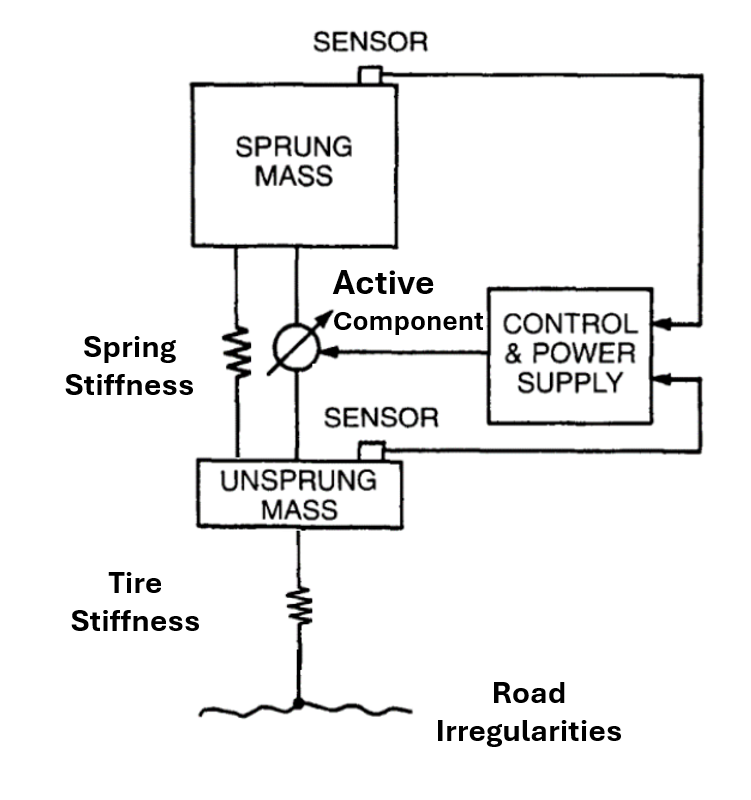
\includegraphics[width=0.4\textwidth]{Active schematic diagram.png}
	\caption{Schematic Diagram of the Modified Active Suspension System \cite{wong2001theory}}
	\label{fig:Active schematic diagram}
	
\end{figure}
\begin{equation}
	M\ddot{z} = -k(z - z_t) - F_a
	\label{eqn:4.2}
\end{equation}

\begin{equation}
	m\ddot{z_t}=-k(z_t-z)-k_t(z_t-z_r)+ F_a
	\label{eqn:4.1}
\end{equation}
\begin{table}[H]
	\centering
	\caption{Parameters of Quarter Car Model \cite{turkay2005study}}
	\begin{tabular}{ l|l }
		\hline
		$M$   & Quarter-car body mass                                              \\
		$m$   & Unsprung mass (Tire, wheel, brake caliper, suspension links, etc.) \\
		$k$   & Stiffness of the suspension                                        \\
		$k_t$ & Stiffness of the tire                                              \\
		$F_a$ &  the control force from the actuator                  \\
		$z$   & Vertical position of the car body                                  \\
		$z_t$ & Vertical position of the unsprung mass                             \\
		$z_r$ & Vertical position of road profile                                  \\
		\hline
	\end{tabular}
	\label{table:qcm}
\end{table}


In this chapter, vehicle dynamic modeling is a major step in the design of suspension systems. According to the requirement of controller design, the three dynamic models: two (DOF) quarter-car models, four DOF half-car models, and seven DOF full-car models, are used for the theoretical analysis and design of suspension systems. \cite{sun2020advanced}
We Explain Types of Road Excitation and the effect of tire radius and how these factors influence of Suspension system Model.

%%%%%%%%%%%%%%%%%%%%%%%%%%%%%%%%

\section{STATE SPACE MODEL}
A state-space representation is a mathematical model used in control theory and system analysis to describe the behavior of a dynamic system. It provides a concise and systematic way to represent the evolution of a system over time. The essential components of a state-space representation include:

\begin{itemize}
	\item State Variables (x): These are variables that describe the current state of the system. They are typically chosen to be the smallest set of variables that completely define the system at any given time.
	\item Input Variables (u): These represent the inputs or control signals applied to the system. Inputs can be manipulated to influence the system's behavior.
	\item Output Variables (y): These represent the measurable outputs of the system. Outputs are influenced by both the current state and the input signals.
	\item State Equations: These are a set of first-order differential equations that describe how the state variables evolve over time. The state equations are often expressed in matrix form as $\dot{x}=Ax+Bu$, where $x$ is the derivative of the state vector $x$, A is the state matrix, B is the input matrix, and u is the input vector.
	\item Output Equations: These equations relate the state and input variables to the output variables. They are typically expressed as $y=Cx+Du$, where $C$ is the output matrix, and $D$ is the feedforward matrix.
\end{itemize}

The state-space representation is particularly useful for analyzing and designing control systems. It allows us to apply linear algebra and matrix theory to study the system's behavior, stability, and controllability. Later, it will help us design controllers that can manipulate inputs to achieve desired system responses \cite{nguyen2023dynamic}, we will use it to represent passive quarter-car model dynamical equations (\ref{eqn:4.1}, \ref{eqn:4.2}), in this chapter we will consider only input in our system is road input $z_r$ as shown in equation \ref{eqn:ssm}, and we neglect $D$  the feedforward matrix in our model.

$$\dot{x}_{(t)}=Ax_{(t)}+Bu_{(t)}$$
$$y_{(t)}=Cx_{(t)}$$
\begin{equation}
	\centering
	\begin{bmatrix}
		\ddot{z}   \\
		\dot{z}    \\
		\ddot{z}_t \\
		\dot{z}_t  \\
	\end{bmatrix}
	=
	\begin{bmatrix}
		-c/M & -k/M & c/M  & k/M        \\
		1    & 0    & 0    & 0          \\
		c/m  & k/m  & -c/m & (-k-k_t)/m \\
		0    & 0    & 1    & 0          \\
	\end{bmatrix}
	\begin{bmatrix}
		\dot{z}   \\
		z         \\
		\dot{z}_t \\
		z_t       \\
	\end{bmatrix}
	+
	\begin{bmatrix}
		0     \\
		z  0  \\
		k_t/m \\
		0     \\
	\end{bmatrix}
	z_r
	\label{eqn:ssm}
\end{equation}
$$
y_{(t)}=
\begin{bmatrix}
	1 & 0 & 0 & 0 \\
	0 & 1 & 0 & 0 \\
	0 & 0 & 1 & 0 \\
	0 & 0 & 0 & 1 \\
	
\end{bmatrix}
\begin{bmatrix}
	\dot{z}   \\
	z         \\
	\dot{z}_t \\image
	z_t       \\
\end{bmatrix}
$$

%%%%%%%%%%%%%%%%%%%%%%%%%%%%%%%%%%%%%%%%%%%%
In this chapter we are going to validate the simulation model by comparing between the simulation results and the experimental results.
\newline
In the simulation results the road input is taken from the road input sensor to ensure the exact behavior in the real world is entered to the simulation model. So, the procedure of the validation is as follows:
\begin{itemize}
	\item Compare the road input of the Slider-Crank mechanism with the road input displacement sensor to ensure the good function of the road input excitation mechanism.
	\item Compare the unsprung mass displacement results either simulation and experimental.
	\item Compare the sprung mass displacement results either simulation and experimental.
\end{itemize}
all these results are repeated three times at different values of excitation frequencies:
\begin{itemize}
	\item 0.309 [Hz]
	\item 0.817 [Hz]
	\item 1.670 [Hz]
\end{itemize}

\section{Road Input Comparison}
\begin{itemize}
	\item 0.309 [Hz]
\end{itemize}
\begin{figure}[H]
	\centering
	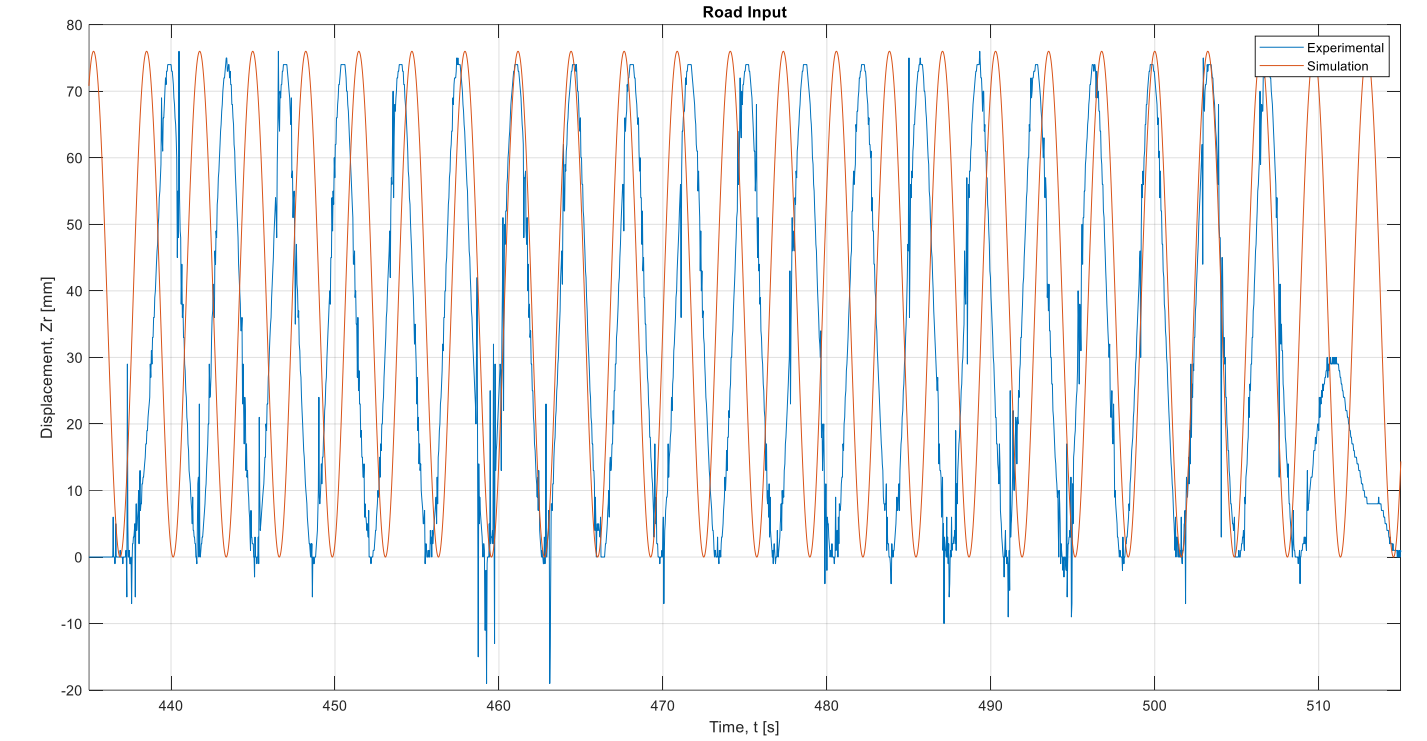
\includegraphics[width=0.9\linewidth]{figures/0.309 RI.png}
	\caption{Road Input Comparison at 0.309 [Hz]}
	\label{fig:Road Input Comparison at 0.309}
\end{figure}

\begin{itemize}
	\item 0.817 [Hz]
\end{itemize}
\begin{figure}[H]
	\centering
	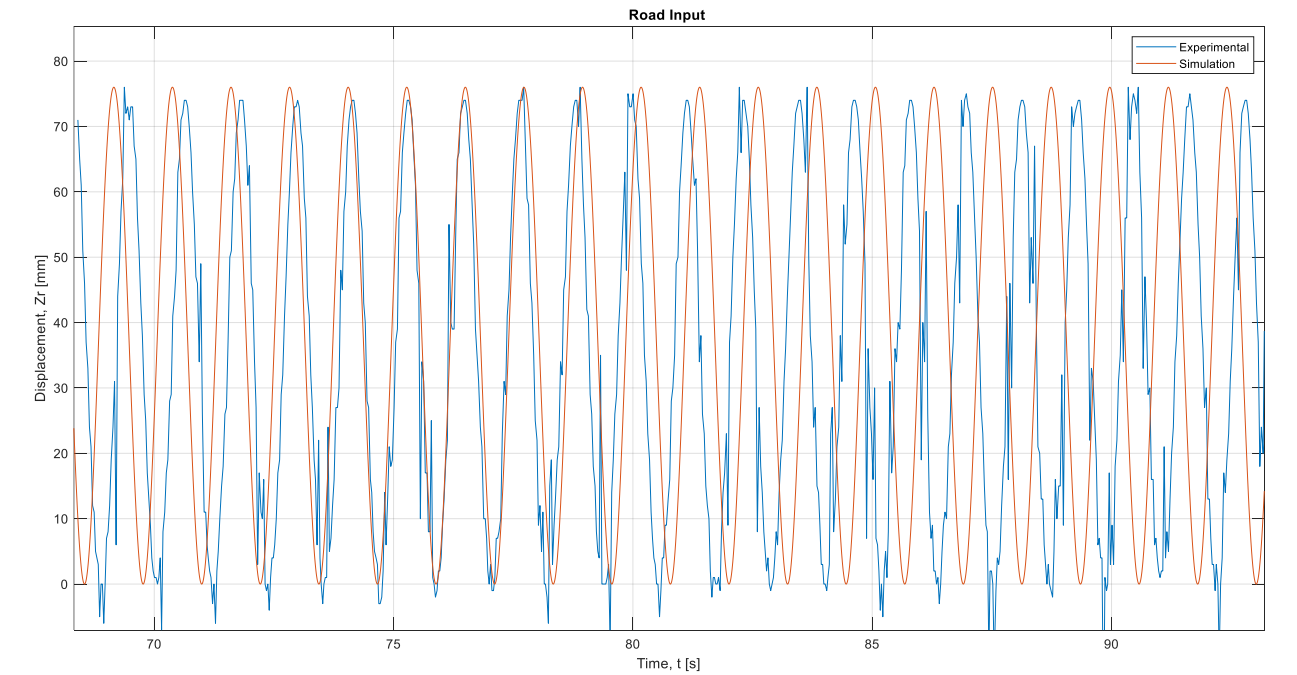
\includegraphics[width=0.99\linewidth]{figures/0.817 RI.png}
	\caption{Road Input Comparison at 0.817 [Hz]}
	\label{fig:Road Input Comparison at 0.817}
\end{figure}
\begin{itemize}
	\item 1.670 [Hz]
\end{itemize}
\begin{figure}[H]
	\centering
	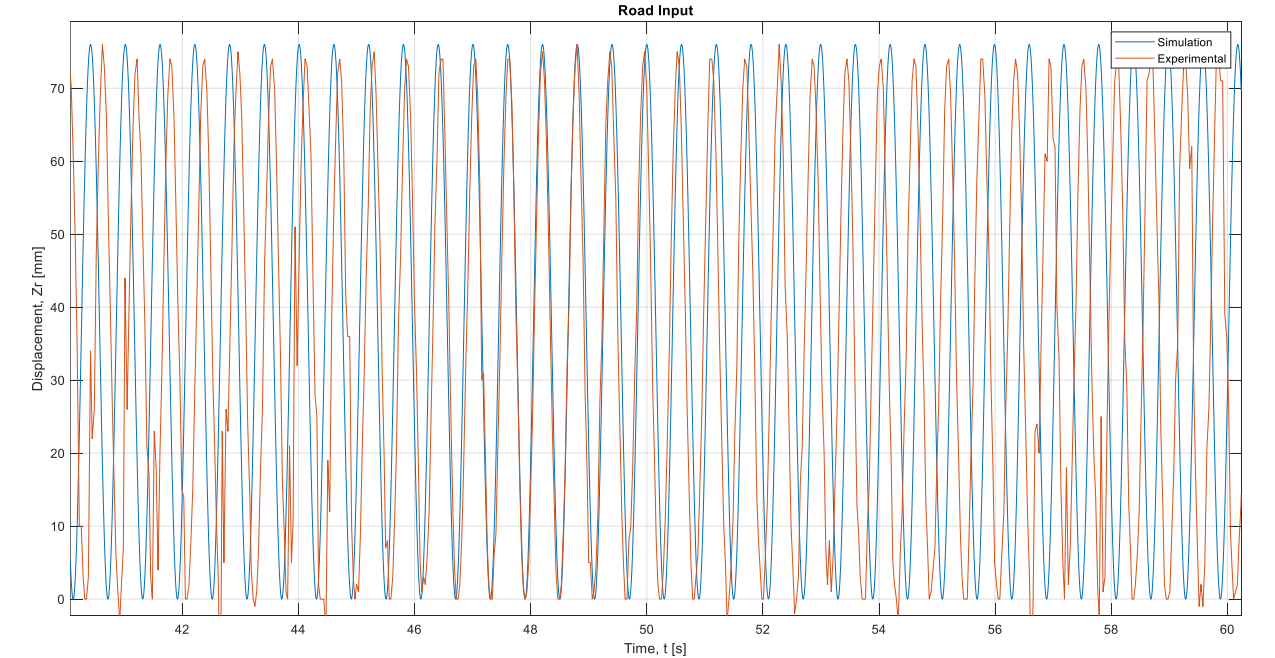
\includegraphics[width=0.99\linewidth]{figures/1.67 RI.png}
	\caption{Road Input Comparison at 1.670 [Hz]}
	\label{fig:Road Input Comparison at 1.670}
\end{figure}


\section{Unsprung mass Displacement Comparison}
\begin{itemize}
	\item 0.309 [Hz]
\end{itemize}
\begin{figure}[H]
	\centering
	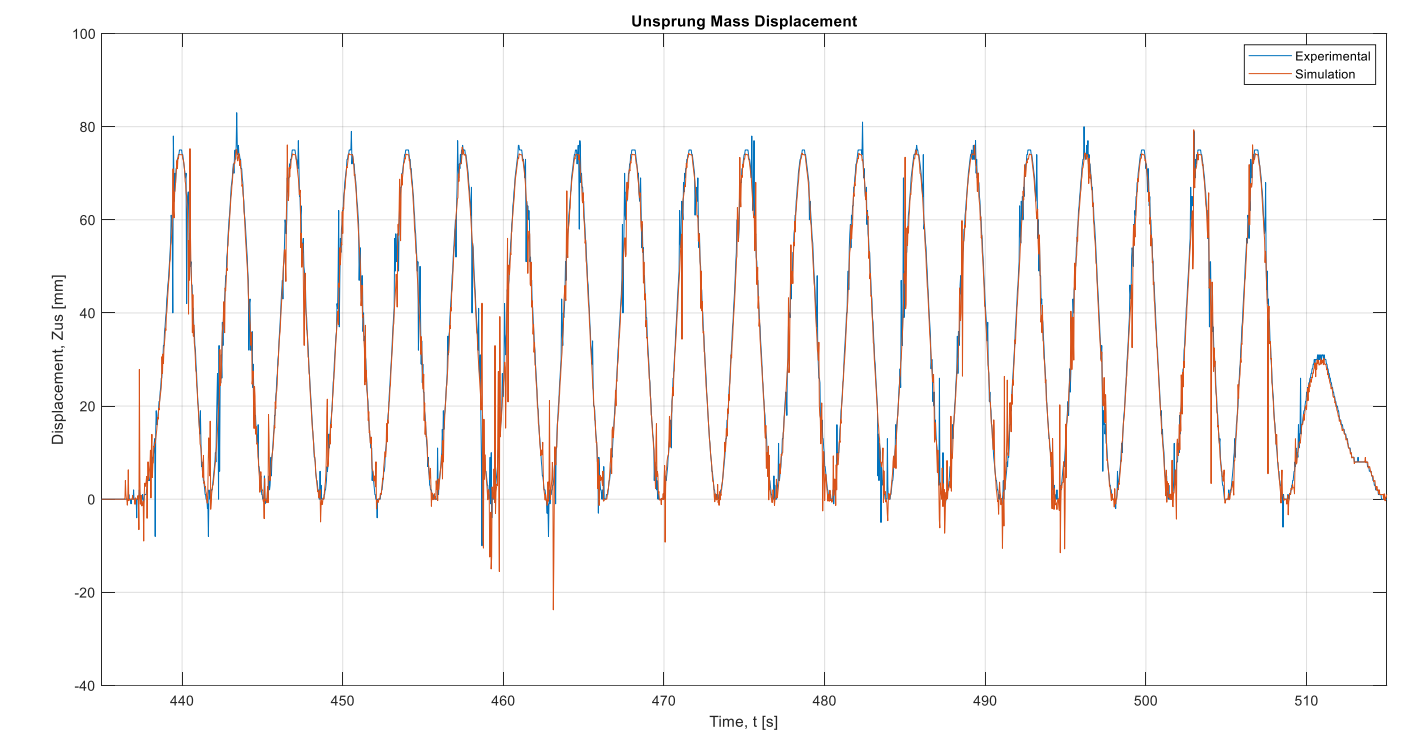
\includegraphics[width=0.9\linewidth]{figures/0.309 Us.png}
	\caption{Unsprung mass Displacement Comparison at 0.309 [Hz]}
	\label{fig:Unsprung mass Displacement Comparison at 0.309}
\end{figure}

\begin{itemize}
	\item 0.817 [Hz]
\end{itemize}
\begin{figure}[H]
	\centering
	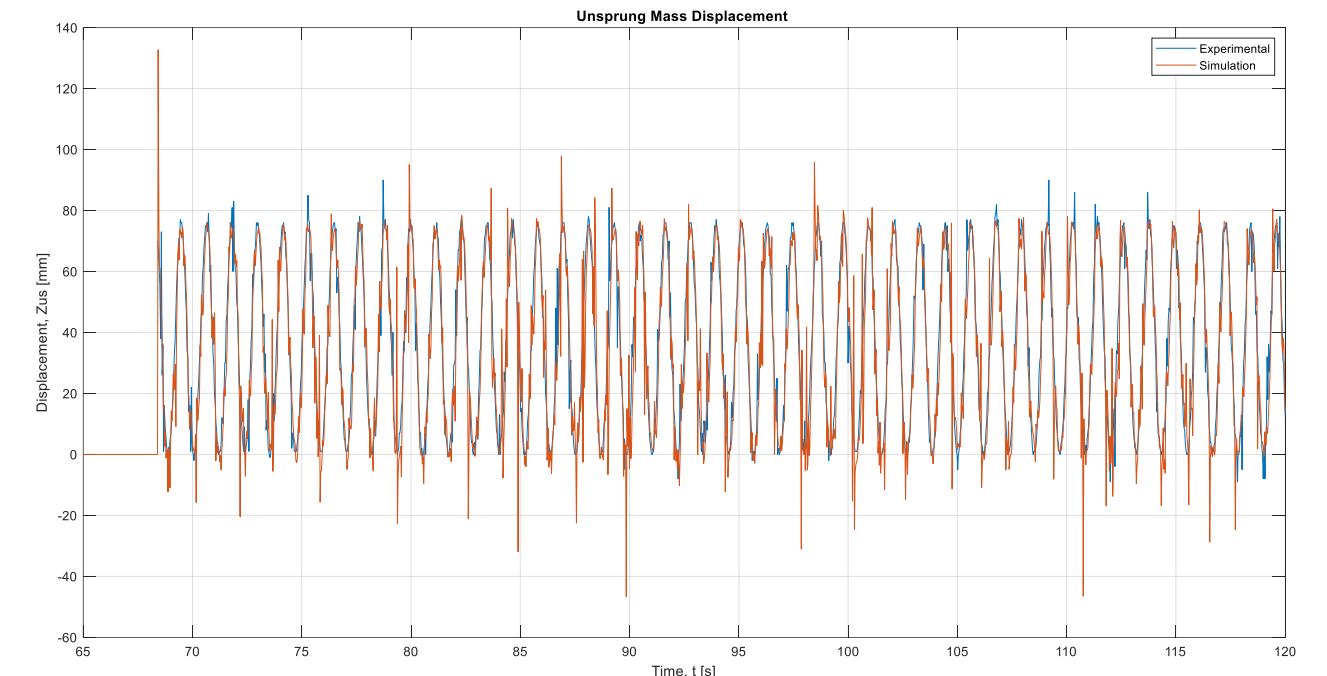
\includegraphics[width=0.99\linewidth]{figures/0.817 Us.png}
	\caption{Unsprung mass Displacement Comparison at 0.817 [Hz]}
	\label{fig:Unsprung mass Displacement Comparison at 0.817}
\end{figure}


\begin{itemize}
	\item 1.670 [Hz]
\end{itemize}
\begin{figure}[H]
	\centering
	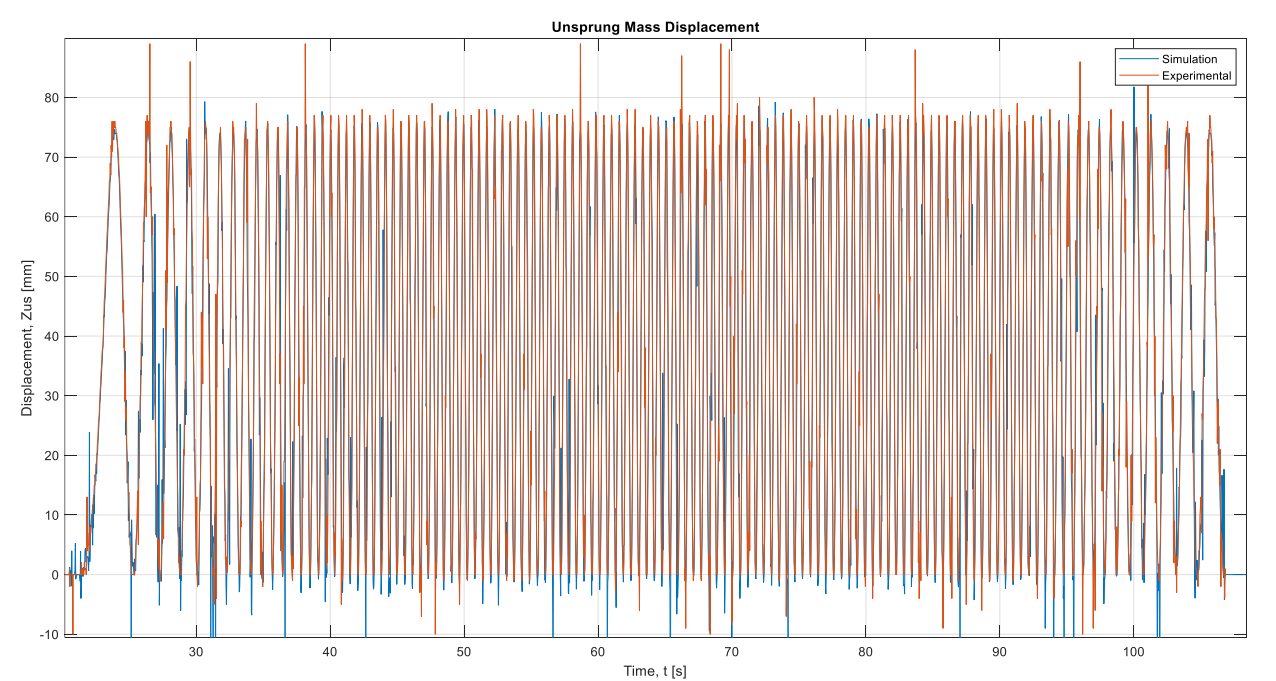
\includegraphics[width=0.99\linewidth]{figures/1.67 Us.png}
	\caption{Unsprung mass Displacement at 1.670 [Hz]}
	\label{fig:Unsprung mass Displacement Comparison at 1.670}
\end{figure}

\section{Sprung mass Displacement Comparison}
\begin{itemize}
	\item 0.309 [Hz]
\end{itemize}
\begin{figure}[H]
	\centering
	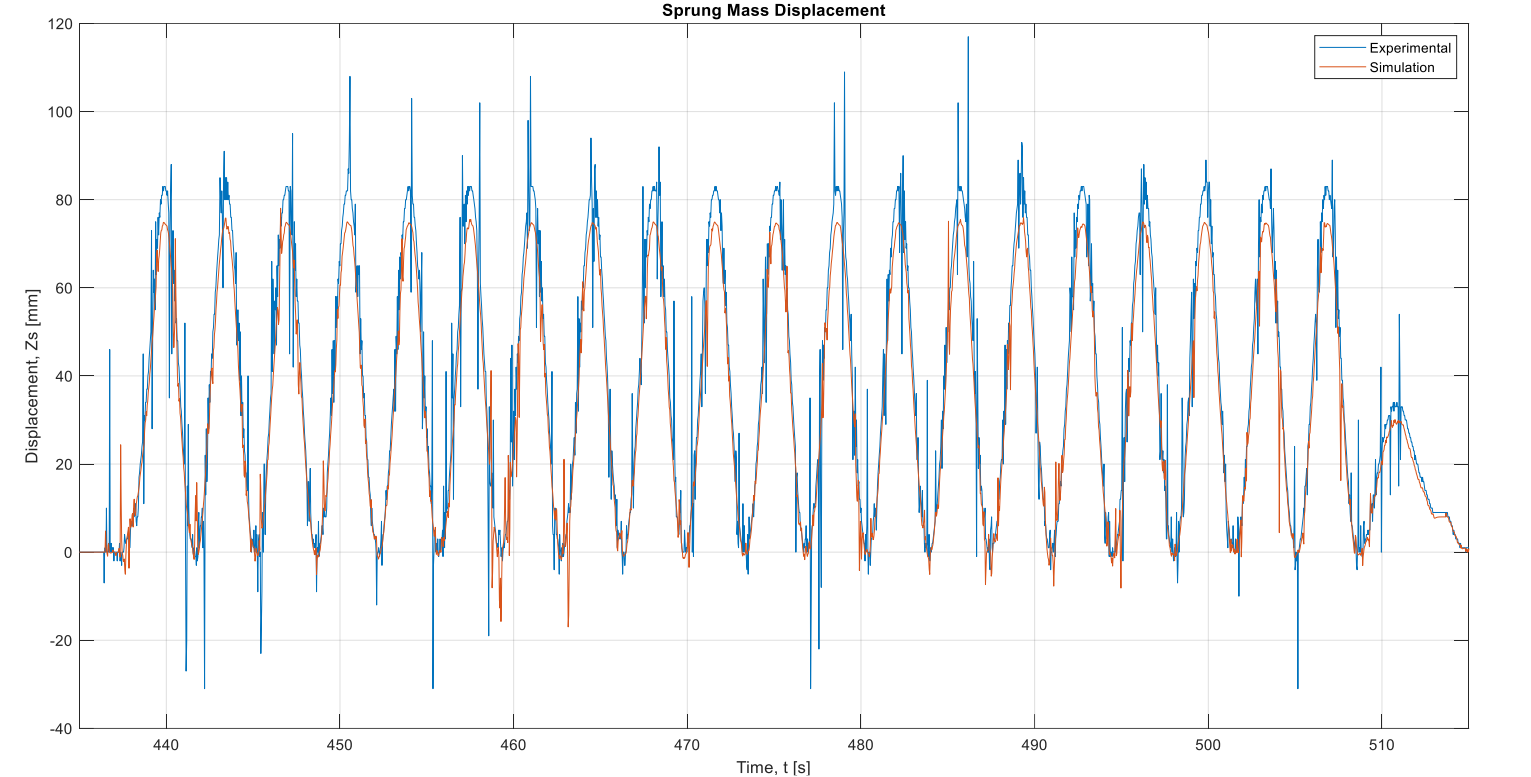
\includegraphics[width=0.9\linewidth]{figures/0.309 S.png}
	\caption{Sprung mass Displacement Comparison at 0.309 [Hz]}
	\label{fig:Sprung mass Displacement Comparison at 0.309}
\end{figure}

\begin{itemize}
	\item 0.817 [Hz]
\end{itemize}
\begin{figure}[H]
	\centering
	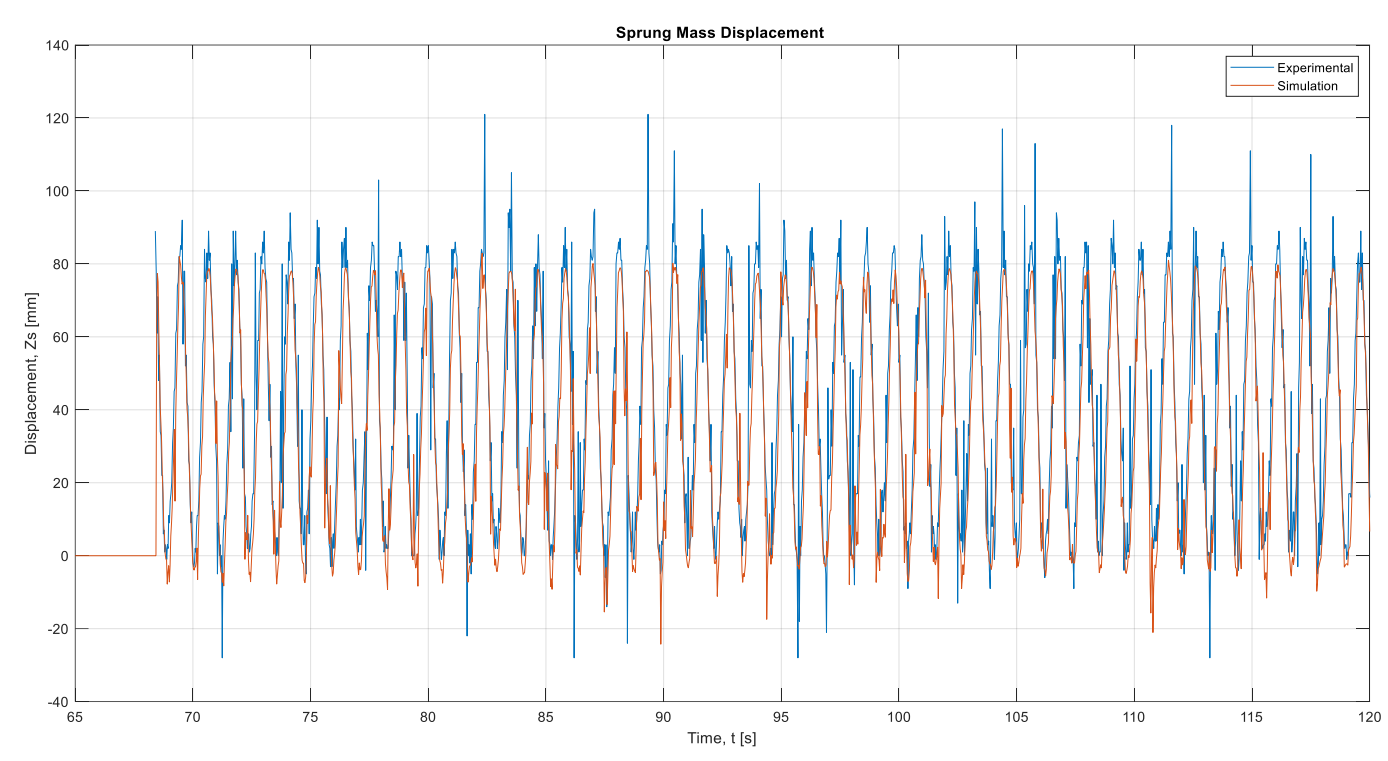
\includegraphics[width=0.99\linewidth]{figures/0.817 S.png}
	\caption{Sprung mass Displacement Comparison at 0.817 [Hz]}
	\label{fig:Sprung mass Displacement Comparison at 0.817}
\end{figure}

\begin{itemize}
	\item 1.670 [Hz]
\end{itemize}
\begin{figure}[H]
	\centering
	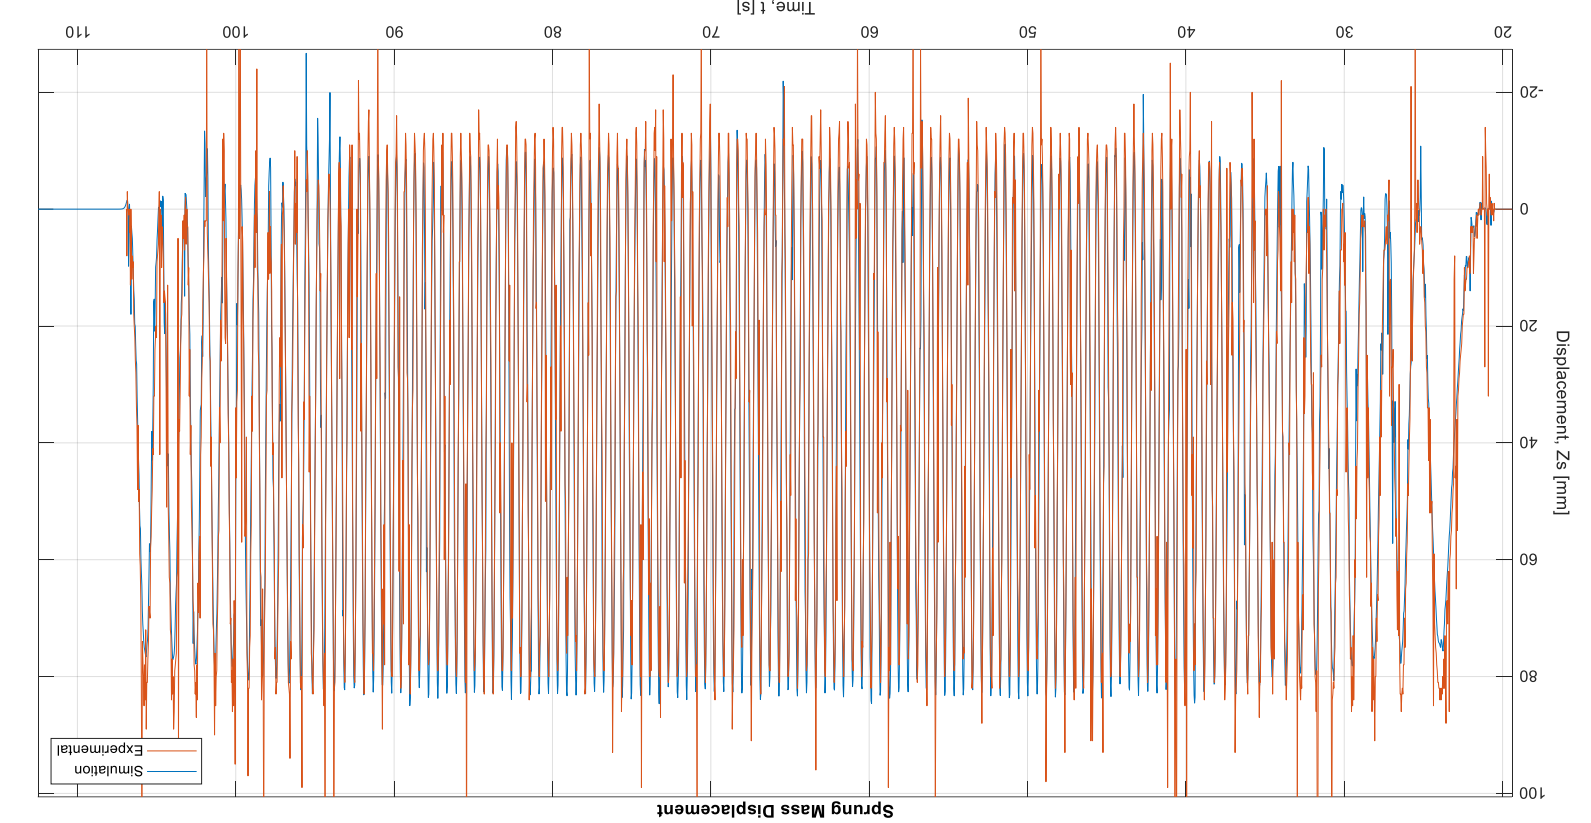
\includegraphics[width=0.99\linewidth]{figures/1.67 S.png}
	\caption{Sprung mass Displacement at 1.670 [Hz]}
	\label{fig:Sprung mass Displacement Comparison at 1.670}
\end{figure}

\section{Conslusion}

As shown in the results above, the simulation model results is very close to the experimental results in the Road Input, Unsprung mass displacement and sprung mass displacement.
\newline
So, the simulation model is valid.
\fi